\section{Discussion}

\subsection{Default Configuration}

The results of the default configuration are shows in Figure \ref{fig:default}.
The default configuration is using four down and up-blocks, and keep the attention layers only at the lowest resolution (bottom) layers to reduce memory usage.
And the model is trained for 300 epochs with a batch size of 32 and time steps of 1000.

\begin{figure}[H]
    \centering
    \begin{subfigure}{0.48\textwidth}
        \centering
        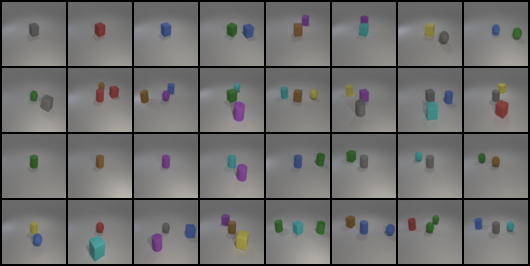
\includegraphics[width=\textwidth]{figures/default_test.png}
        \caption{Default Configuration Results on Test Set with accuracy of 0.9010}
        \label{fig:default_test}
    \end{subfigure}
    \hfill
    \begin{subfigure}{0.48\textwidth}
        \centering
        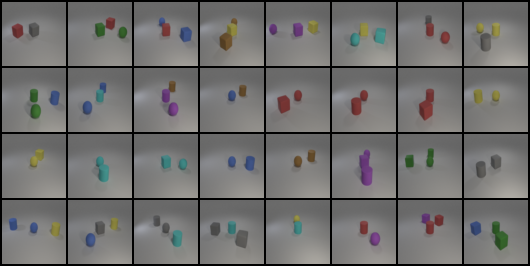
\includegraphics[width=\textwidth]{figures/default_new_test.png}
        \caption{Default Configuration Results on New Test Set with accuracy of 0.9271}
        \label{fig:default_new_test}
    \end{subfigure}
    \caption{Default Configuration Results and Accuracy}
    \label{fig:default}
\end{figure}

And the results of the manual test with ``red sphere'', ``cyan cylinder'', and ``cyan cube'' are shown in Figure \ref{fig:default_manual}.
\begin{figure}[H]
    \centering
    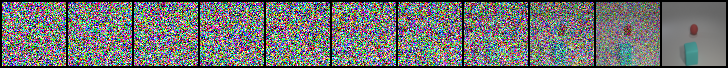
\includegraphics[width=\textwidth]{figures/default_manual_test.png}
    \caption{Default Configuration Results on Manual Test Set with accuracy of 1.0000}
    \label{fig:default_manual}
\end{figure}

And the loss curve of the default configuration is shown in Figure \ref{fig:loss_curve}.

\subsection{Same model with different time steps}

\subsubsection{500 Time Steps}
The results of the same model with different time steps are shown in Figure \ref{fig:step_500}.
The model is trained for 300 epochs with a batch size of 32 and time steps of 500.
\begin{figure}[H]
    \centering
    \begin{subfigure}{0.48\textwidth}
        \centering
        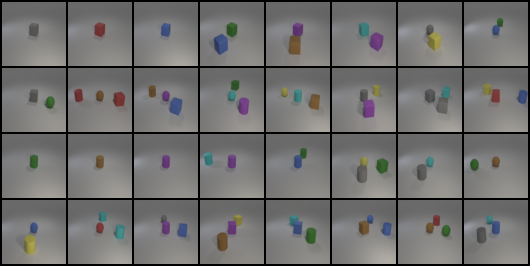
\includegraphics[width=\textwidth]{figures/step_500_test.png}
        \caption{500 Time Steps Results on Test Set with accuracy of 0.9740}
        \label{fig:step_500_test}
    \end{subfigure}
    \hfill
    \begin{subfigure}{0.48\textwidth}
        \centering
        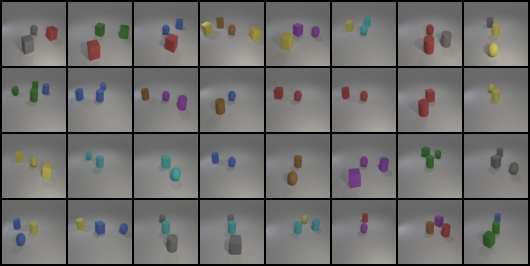
\includegraphics[width=\textwidth]{figures/step_500_new_test.png}
        \caption{500 Time Steps Results on New Test Set with accuracy of 0.8906}
        \label{fig:step_500_new_test}
    \end{subfigure}
    \caption{500 Time Steps Results and Accuracy}
    \label{fig:step_500}
\end{figure}

And the results of the manual test with ``red sphere'', ``cyan cylinder'', and ``cyan cube'' are shown in Figure \ref{fig:step_500_manual}.

\begin{figure}[H]
    \centering
    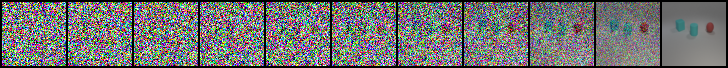
\includegraphics[width=\textwidth]{figures/step_500_manual_test.png}
    \caption{500 Time Steps Results on Manual Test Set with accuracy of 1.0000}
    \label{fig:step_500_manual}
\end{figure}
And the loss curve of the 500 time steps is shown in Figure \ref{fig:loss_curve}.

\subsubsection{100 Time Steps}

The results of the same model with different time steps are shown in Figure \ref{fig:step_100}.
The model is trained for 300 epochs with a batch size of 32 and time steps of 100.

\begin{figure}[H]
    \centering
    \begin{subfigure}{0.48\textwidth}
        \centering
        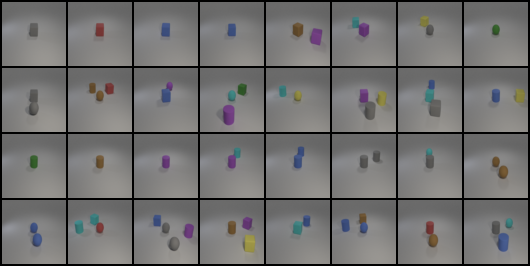
\includegraphics[width=\textwidth]{figures/step_100_test.png}
        \caption{100 Time Steps Results on Test Set with accuracy of 0.8021}
        \label{fig:step_100_test}
    \end{subfigure}
    \hfill
    \begin{subfigure}{0.48\textwidth}
        \centering
        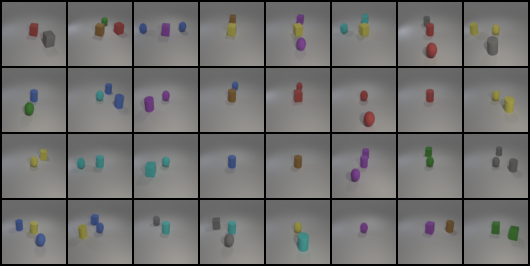
\includegraphics[width=\textwidth]{figures/step_100_new_test.png}
        \caption{100 Time Steps Results on New Test Set with accuracy of 0.7865}
        \label{fig:step_100_new_test}
    \end{subfigure}
    \caption{100 Time Steps Results and Accuracy}
    \label{fig:step_100}
\end{figure}

And the results of the manual test with ``red sphere'', ``cyan cylinder'', and ``cyan cube'' are shown in Figure \ref{fig:step_100_manual}.
\begin{figure}[H]
    \centering
    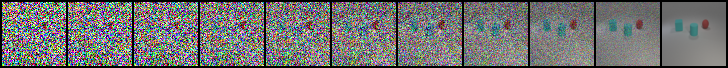
\includegraphics[width=\textwidth]{figures/step_100_manual_test.png}
    \caption{100 Time Steps Results on Manual Test Set with accuracy of 1.0000}
    \label{fig:step_100_manual}
\end{figure}

And the loss curve of the 100 time steps is shown in Figure \ref{fig:loss_curve}.

\subsection{Discussion of Results}

The results of the default configuration and the same model with different time steps are shown in Figure \ref{fig:loss_curve}.
The model with 1000 time steps has the lowest loss, and the model with 500 or 100 time steps has a higher loss.
We can see that the more time steps we have, the lower the loss is.


\begin{figure}[H]
    \begin{tikzpicture}
        \begin{axis}[
                title={Loss Curve of Default Configuration},
                xlabel={Epoch},
                xmin=0,
                xmax=300,
                ymode=log,
                ylabel={Loss},
                grid=major,
                width=\textwidth,
                height=0.5\textwidth,
                cycle list name=color list,
            ]
            \addplot table[col sep=comma, x=Step, y=Value] {csvs/default.csv};
            \addlegendentry{Train Loss with 1000 Time Steps}
            \addplot table[col sep=comma, x=Step, y=Value] {csvs/step-500.csv};
            \addlegendentry{Train Loss with 500 Time Steps}
            \addplot table[col sep=comma, x=Step, y=Value] {csvs/step-100.csv};
            \addlegendentry{Train Loss with 100 Time Steps}
            \addplot table[col sep=comma, x=Step, y=Value] {csvs/large.csv};
            \addlegendentry{Train Loss with 1000 Time Steps (Large Model)}
        \end{axis}
    \end{tikzpicture}
    \caption{Loss Curve of Different Time Steps}
    \label{fig:loss_curve}
\end{figure}

\subsection{Larger Model}

I also tried to use 6 down and up-blocks, and keep the attention layers only at the lowest two resolution (bottom) layers to reduce memory usage.
The model is trained for 300 epochs with a batch size of 32 and time steps of 1000.

Since the results shows similar with the previous model, I didn't include the results here.
But I will include the loss curve of the larger model.
The loss curve is shown in Figure \ref{fig:loss_curve_large}.
